\documentclass[12pt]{article}%
\usepackage{amsfonts}
\usepackage{fancyhdr}
\usepackage{comment}
\usepackage[a4paper, top=2.5cm, bottom=2.5cm, left=2.2cm, right=2.2cm]%
{geometry}
\usepackage{times}
\usepackage{amsmath}
\usepackage{changepage}
\usepackage{amssymb}
\usepackage{graphicx}%
\setcounter{MaxMatrixCols}{30}
\newtheorem{theorem}{Theorem}
\newtheorem{acknowledgement}[theorem]{Acknowledgement}
\newtheorem{algorithm}[theorem]{Algorithm}
\newtheorem{axiom}{Axiom}
\newtheorem{case}[theorem]{Case}
\newtheorem{claim}[theorem]{Claim}
\newtheorem{conclusion}[theorem]{Conclusion}
\newtheorem{condition}[theorem]{Condition}
\newtheorem{conjecture}[theorem]{Conjecture}
\newtheorem{corollary}[theorem]{Corollary}
\newtheorem{criterion}[theorem]{Criterion}
\newtheorem{definition}[theorem]{Definition}
\newtheorem{example}[theorem]{Example}
\newtheorem{exercise}[theorem]{Exercise}
\usepackage{hyperref}
\usepackage{minted}
\newtheorem{lemma}[theorem]{Lemma}

\newtheorem{notation}[theorem]{Notation}
\newtheorem{problem}[theorem]{Problem}
\newtheorem{proposition}[theorem]{Proposition}
\newtheorem{remark}[theorem]{Remark}
\newtheorem{solution}[theorem]{Solution}
\newtheorem{summary}[theorem]{Summary}
\newenvironment{proof}[1][Proof]{\textbf{#1.} }{\ \rule{0.5em}{0.5em}}

\newcommand{\Q}{\mathbb{Q}}
\newcommand{\R}{\mathbb{R}}
\newcommand{\C}{\mathbb{C}}
\newcommand{\Z}{\mathbb{Z}}

\begin{document}

\title{Homework Assignment 1}
\author{COGS 181: Neural Networks and Deep Learning}
\date{}
\maketitle

\noindent \textbf {Due: Oct. 6, 2017, 11:59pm } \\
\noindent \textbf {Instructions:} Please answer the questions below, attach your code, and insert figures to create a pdf file; submit your file to TED (ted.ucsd.edu) by 11:59pm, 10/06/2017. You may search information online but you will need to write code/find solutions to answer the questions yourself.\\

\noindent \textbf{Late Policy:} \%5 of the total points will be deducted on the first day past due. Every 10\% of the total points will be deducted for every extra day past due.\\

\noindent \textbf{System Setup:} You are free to choose either pip or anaconda as the package installer. After the installation of one of the installer, type pip/conda install \$PACKAGE\_NAME in the terminal to install python packages. For more information, see Piazza system setup post.\\

\noindent Grade: \underline{\hspace{.8cm}} out of 100 points \\
\section{(15 points)Basic Matrix Operations Using Numpy}
Suppose $\mathbf{A}=\begin{bmatrix}
1&3 \\
5&7 \\
9&11 \\
\end{bmatrix}$, 
$\mathbf{B}=\begin{bmatrix}
1 & -1 \\
-1 & 1 \\
-1 & 0 \\
\end{bmatrix}$, we can convert $\mathbf{A}$ and $\mathbf{B}$ into numpy arrays by
\begin{minted}{python}
import numpy as np
A = np.array([[1,3],[5,7],[9,11]])
B = np.array([[1,-1],[-1,1],[-1,0]])
\end{minted}
Numpy package uses np.dot(A,B) to compute the dot product between matrices A and B. Binary operators such as '*','/','+' and '-' compute the element-wise operations between two matrices. Please compute the following: (If the matrix multiplication is not possible, write 'impossible' in your answer)
\begin{enumerate}
\item $A-B$
\item $A\circ B$ (element-wise product)
\item $A^TB$
\item $AB^T$
\item $AB$
\end{enumerate}
\vspace{30mm}

\section{(20 points)Basic Plots Using Matplotlib}
Matplotlib is a very useful library to plot graphs. In later course, you may need to plot your own graphs such as: losses v.s. iterations, accuracies v.s. categories and include those graphs in your report. We will start with a simple exercise. Copy and paste the following code into one notebook cell:
\begin{minted}{python}
import matplotlib.pyplot as plt
%matplotlib inline
np.random.seed(0)
space = np.linspace(0,10,num=50)
sine = np.sin(space)
plt.scatter(space,sine,color='b',label = 'sine_curve')
sine_5 = sine
for i in range(5):
    sine_5 = sine_5 + np.random.normal(scale=0.1,size=50)
plt_sine_5, = plt.plot(space,sine_5,color='r',label = 'noise_5_iters')
plt.legend(loc='upper right')
plt.savefig('./cogs181_Q2.png')
\end{minted}
The above code creates a graph with the original sine curve and another curve which 5 iterations of Gaussian noise (0 mean, 0.1 standard deviation) are added to the original sine curve. You should get a graph similar like this:
\begin{figure}[!htp]
\begin{center}
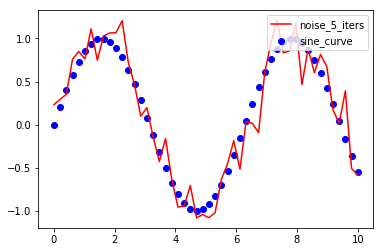
\includegraphics[width=0.5\linewidth]{Q2.png} 
\label{fig:Q2}
\end{center}
\end{figure}\\
Edit the code above and apply 20 and 100 iterations of Gaussian noise (0 mean, 0.1 standard deviation) on the original sine curve respectively. Plot all four curves in one graph (including the two curves from the original code) and add the legend of the additional curves and label them as 'noise\_20\_iters' and 'noise\_100\_iters'.
\vspace{50mm}

\section{(25 points)Basic Image Operations Using Scipy}
Scipy library offers a variety of functions for common image processing. In this section you will load the image, resize image and rotate image. First you need to install scipy and download the image 'tabby.jpg' from our course website.

\begin{minted}{python}
from scipy.misc import imread 
img = imread(/path/to/image)
\end{minted}
Complete the following questions and paste your output in the homework:
\begin{enumerate}
\item What is the shape of the image array?(hint: 3 dimensions)
\item Resize the image to 300x300 using scipy.misc.imresize
\end{enumerate}
Besides resize, we are also interested in rotating images and \href{https://docs.scipy.org/doc/scipy-0.19.1/reference/ndimage.html}{scipy.ndimage} provides more image operations than scipy.misc.
\begin{minted}{python}
from scipy.misc import imread 
img = imread(/path/to/image)
from scipy.ndimage import rotate 
rotated = rotate(img,30,reshape=False,mode='nearest',cval=0)
\end{minted}
Complete the following questions and paste your output in the homework. All the operations should base on the original image ('img' in the code):
\begin{enumerate}
\item Set the reshape option to True
\item Change the mode to 'constant', and let 'cval' be 0 
\item Change the mode to 'constant', and let 'cval' be 255
\item Change the mode to 'reflect'
\end{enumerate}
\vspace{30mm}

\section{(15 points) Data and Visualization}
%Download the Iris Data Set from UCI Machine Learning Repository (click \href{http://archive.ics.uci.edu/ml/machine-learning-databases/iris/iris.data}{\textbf{\emph{here}}}).\\
%http://archive.ics.uci.edu/ml/machine-learning-databases/iris/iris.data). \\
The dataset description can be found \href{https://archive.ics.uci.edu/ml/datasets/Iris}{\textbf{\emph{here}}}.\\
https://archive.ics.uci.edu/ml/datasets/Iris.\\
Plot two figures to visualize the dataset using: (1) the first 2 feature dimensions, and (2) the first 3 feature dimensions. Some useful instructions are shown below: \\
%%%python for Q1
\textbf{Python:}
\begin{enumerate}
\item[{(1)}] Import several useful package into Python:
\begin{minted}{python}
import matplotlib.pyplot as plt
from sklearn import datasets
from mpl_toolkits.mplot3d import Axes3D
\end{minted}
\item[{(2)}] Load Iris dataset into Python:
\begin{minted}{python}
iris = datasets.load_iris()
X = iris.data
Y = iris.target
\end{minted}
\item[{(3)}] Visualize first 2 feature dimensions:
\begin{minted}{python}
plt.scatter(X[:,0],X[:,1], c=Y, cmap=plt.cm.Paired)
\end{minted}
\item[{(4)}] Visualize first 3 feature dimensions:
\begin{minted}{python}
fig = plt.figure(1, figsize=(8, 8))
ax = Axes3D(fig, elev=-150, azim=110)
ax.scatter(X[:,0],X[:,1],X[:,2],c=Y,cmap=plt.cm.Paired)
\end{minted}
\end{enumerate}
\vspace{30mm}

\section{(10 points) One-hot Encoding}
A dataset $S$ is denoted as $S=\{{\bf x}_1,{\bf x}_2,{\bf x}_3,{\bf x}_4,{\bf x}_5 \}$, where each sample refers to the specification of a car.

\begin{table}[!h]
\begin{center}
\begin{tabular}{l|||c|c|c|}
 & Length (inch) & Height (inch) & Color \\
\hline
${\bf x}_1$ & 182.3 & 62 & Silver \\
 \hline
 ${\bf x}_2$ & 181 & 66 & Blue  \\
  \hline
${\bf x}_3$ & 186 & 56 & Red  \\
  \hline
 ${\bf x}_4$ & 179 & 59 & Blue  \\
  \hline
 ${\bf x}_5$  & 182 & 50 & Black  \\
\hline
\end{tabular}
\end{center}
\end{table}
Please represent this dataset $S$ using a matrix and show it below. 
{\bf Hint}: for the categorical feature, you may use the one-hot encoding strategy; you can choose either a row vector or a column vector to represent each data sample, but please use one consistently for the entire dataset.

\vspace{50mm}

\section{(15 points) Linear regression}
Download the data file \textbf{data.txt} from the course website: \href{}{data.txt}\\ and load the data into your environment. The data samples are represented as row vectors; the first column refers to the input (x-axis) and the second column refers to the output (y-axis). We assume that this dataset was generated from a linear model: $y=ax+b$ plus noise, and you need to find the optimal $a^*$ and $b^*$ to fit the data. Now follow the instructions below using the least squre estimation and show the result in your report. \\
\newline
\textbf{HINT:}
The closed form solution for the least square estimation is $W =(X^TX)^{-1}X^TY$.\\
\textbf{Python:}
\begin{enumerate}
\item[{(1)}] Import $matplotlib$ and $numpy$ package into Python.
\begin{minted}{python}
import matplotlib.pyplot as plt
import numpy as np
\end{minted}
\item[{(2)}] Load data.
\begin{minted}{python}
data = np.loadtxt('data.txt',dtype='float')
x = data[:,0].reshape(len(data),1)
y = data[:,1].reshape(len(data),1)
\end{minted}
\item[{(3)}] Plot the data.
\begin{minted}{python}
plt.plot(x,y)
plt.grid()
\end{minted}
\item[{(4)}] Create the matrix
\begin{minted}{python}
X = np.hstack((np.ones((len(x),1)),np.power(x,1)))
\end{minted}
\item[{(5)}] Compute the least squares line over the given data by
\begin{minted}{python}
X_t = X.transpose((1,0))
sol = np.dot(np.linalg.inv(np.dot(X_t,X)),np.dot(X_t,y))
\end{minted}
\item[{(6)}] Plot the least square line, and assign title to the figure
\begin{minted}{python}
plt.plot(x,y)
plt.hold(True)
plt.plot(x,sol[0]+sol[1]*x)
plt.title('Least square line fitting')
plt.xlabel('x')
plt.ylabel('y')
\end{minted}
\end{enumerate}

\end{document}